
\def\columnseprulecolor{\color{ocre}}
\setlength{\columnseprule}{0.4pt} 

\begin{multicols}{2}

%
%\begin{center}
%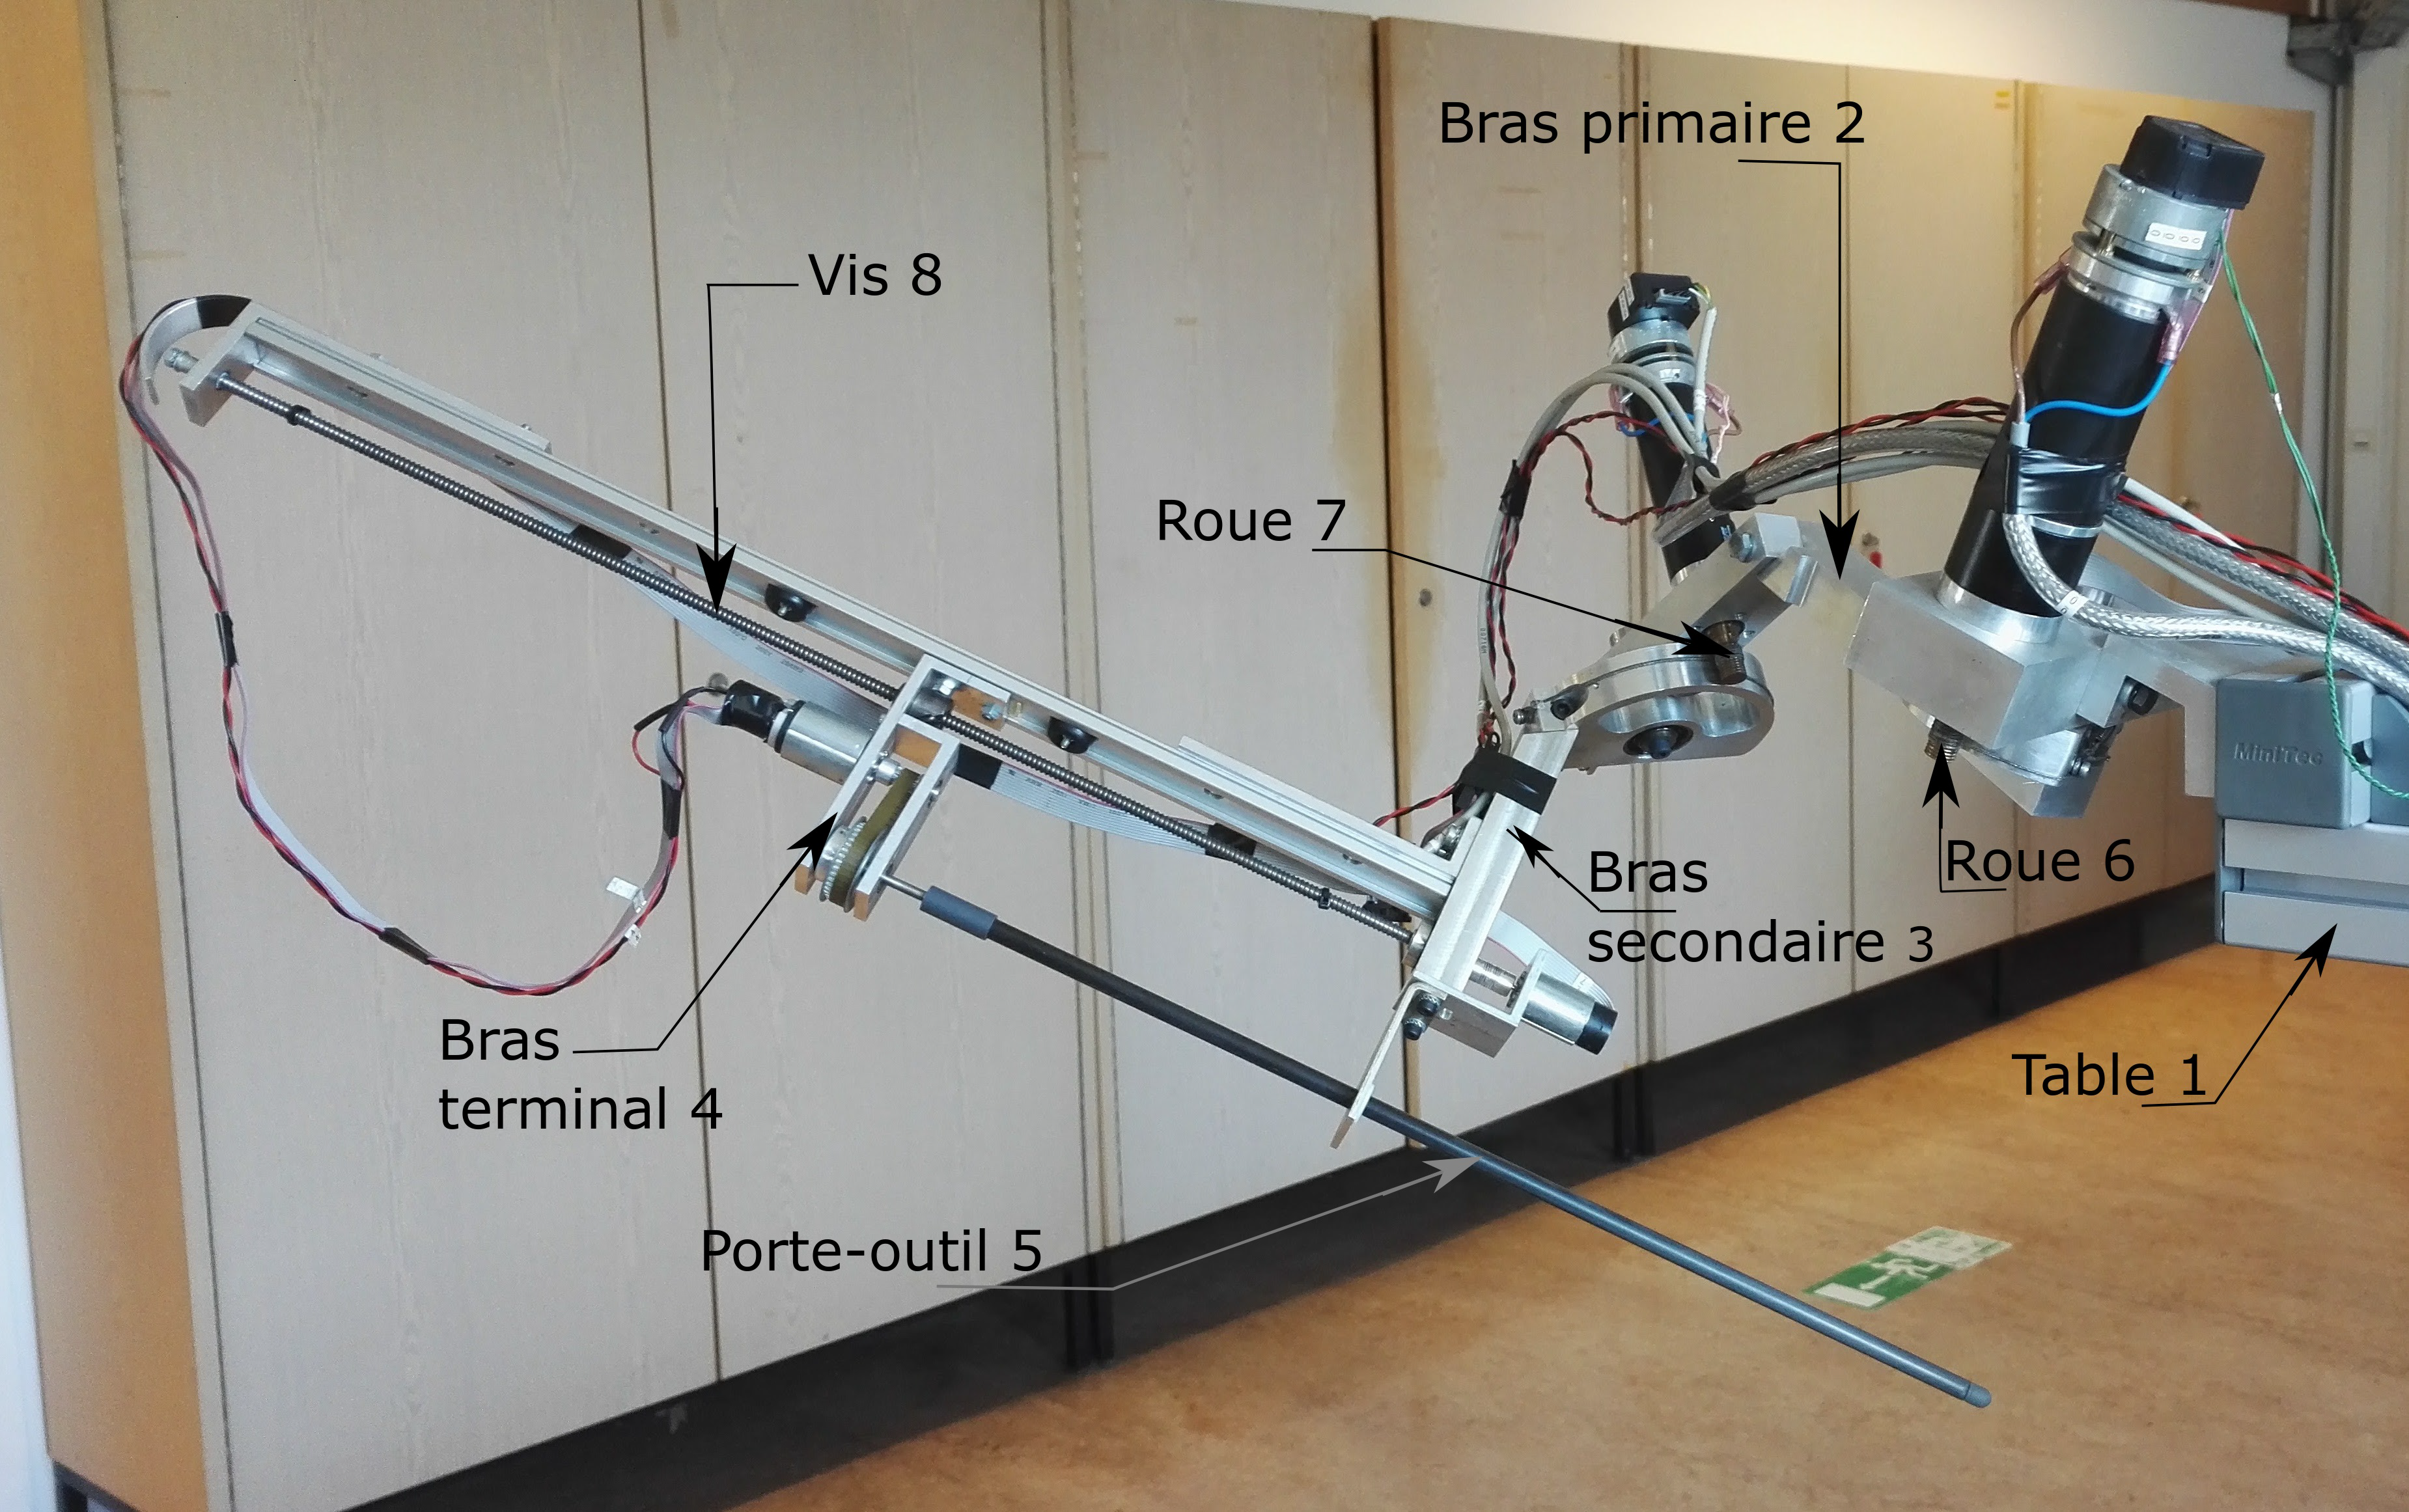
\includegraphics[width=\linewidth]{images/fig_00}
%\end{center}
\footnotesize
Le sujet porte sur la modélisation de la loi de commande en protection d’incidence dans le cas du vol longitudinal d’un avion de type Airbus A350 XWB.


Ce biréacteur gros porteur et moyen-long courrier, dernier né de la famille du constructeur européen Airbus et mis en service en janvier 2015, a été baptisé « A350 XWB », pour eXtraWide Body (fuselage extra large).


Cette nouvelle génération d’avion comporte 3 versions passagers qui ont un rayon d’action complémentaire :

\begin{center}
\begin{tabular}{|p{1.9cm}|c|c|c|}
\hline
Spécifications & A350-800 & A350-900 & A350-1000 \\ \hline
Longueur	& \SI{60,54}{m} & \SI{66,89}{m} & \SI{73,78}{m} \\ \hline
Envergure	& \SI{64,75}{m}&	\SI{64,91}{m}&	\SI{64,75}{m} \\ \hline
Largeur fuselage	& \SI{5,96}{m}&	\SI{5,96}{m}&	\SI{5,96}{m} \\ \hline
Hauteur	& \SI{17,05}{m}&\SI{17,05}{m}&\SI{17,08}{m} \\ \hline
Capacité en sièges	& 276& 315	&369 \\ \hline
Distance franchissable	& \SI{15 300}{km}& 	\SI{14 350}{km}	&\SI{14 800}{km} \\ \hline
Masse au décollage		& \SI{248}{t}	&\SI{268}{t}	& \SI{308}{t} \\ \hline
Capacité des réservoirs	& \SI{138 000}{L}& \SI{138 000}{L}&\SI{156 000}{L} \\ \hline
Poussée des moteurs	& \SI{337}{kN} & \SI{374}{kN}  &\SI{442}{kN} \\ \hline
 &  & Mach 0,89 &  \\ 
Vitesse maximale en Mach 
\footnote{Mach 1 = $\SI{1234,8}{km.h^{-1}}= \SI{340}{m.s^{-1}}$ 
(vitesse du son dans l’air à 0\degres C).} 
&  & \SI{593,40}{kt}
\footnote{kt : milles nautiques par heure (knot en anglais) -- $\SI{1}{kt}= \SI{1,852}{km.h^{-1}} = \SI{0,514}{m.s^{-1}}$}. &  \\ 
 &  & \SI{305,27}{m.s^{-1}} &  \\ \hline
%en kt	(2)
%	   en m.s-1	Mach 0,89
%593,40 kt
%305,27 m.s-1
\end{tabular}
\end{center}
\normalsize


La principale prouesse technologique réside dans la réduction de consommation de kérosène de plus de 25\% par rapport à la gamme A340. Ceci grâce à l’emploi de matériaux composite innovant plus légers (fibre de carbone renforcée de plastique -- voilure et fuselage).


\section*{Présentation et plan de l'étude}
L’étude fera référence à des termes définis dans les documents DOC 1 et DOC 2 des.	Il est vivement conseillé de consulter ces documents avant de commencer le sujet.


Le schéma de la Figure 1, illustre les différentes boucles de commande rencontrées sur la commande de vol de l’A350 XWB.

Les lois de commande de vol, linéaires ou non, doivent être robustes et embarquables dans les calculateurs d’avions de transport modernes. Nous nous intéresserons dans ce sujet à une phase de vol longitudinal, exigeante car en transitoire et à proximité du sol : manœuvre d’évitement instinctive (avoidance carefree maneuver).

Le sujet comporte 3 parties indépendantes.

Pour commencer, la partie A s’intéresse à la description du modèle avion rigide afin d’appréhender les lois de pilotage d’un avion.

Le contrôle de l’avion suivant l’axe de tangage s’effectue en contrôlant trois surfaces mobiles horizontales à l’arrière de l’appareil : 2 gouvernes de profondeur et 1 plan horizontal réglable PHR.
Les gouvernes de profondeur assurent la commande longitudinale à court terme, alors que le PHR assure la commande longitudinale à long terme (constante de temps de l’ordre de \SI{14}{s}) permettant de conserver un braquage de la profondeur en moyenne nulle.
Dans le but de contrôler l’avion dans une phase dynamique, nous analyserons le comportement des gouvernes de profondeur dans la partie B.

L’état de l’avion est mesuré par les ADIRS (\textit{Air Data and Inertial Reference System}). Le calculateur embarqué reçoit trois valeurs redondantes pour chaque paramètre de vol et doit élaborer une seule et unique valeur pour le calcul des commandes. Ce point sera abordé en introduction de la partie C, dans le cas particulier des capteurs d’incidence (sondes). L’étude se poursuivra, par la mise en place d’un correcteur pour l’ensemble des boucles d’asservissements (boucles 1 à 5). La conclusion de cette partie C permettra de vérifier les performances attendues en termes de qualité de vol.

\section*{Partie A -- Conduite de vol longitudinal}
\subsection*{I -- Vol symétrique}
\begin{obj}
Mettre en place les conditions du vol longitudinal pur afin de proposer un paramétrage simplifié.
\end{obj}
\begin{center}
\includegraphics[width=\linewidth]{images/fig_01}
\textit{Figure 1 : les différentes boucles de contrôle mises en jeu dans la commande de vol.}
\end{center}

Pour mettre en œuvre les équations du vol, nous définirons trois repères (voir DOC 2). Le repère terrestre supposé galiléen, le repère avion ainsi que le repère aérodynamique.

\subsubsection*{Vol symétrique}
Un vol sera qualifié de symétrique lorsque l’écoulement de l’air est parallèle au plan de symétrie de l’avion $(G, \vect{x_b},\vect{z_b})$.

Supposons que l’avion en vol symétrique subisse une rafale provenant de la gauche. Cette situation amène l’axe longitudinal de l’avion à se placer dans le lit du vent correspondant à la rafale. L’avion est alors dit en dérapage à droite (voir Figure 2).


\begin{center}
\includegraphics[width=\linewidth]{images/fig_02}
\textit{Figure 2 Avion en dérapage à droite}
\end{center} 


{\begin{question}{q01}
Quelle est la conséquence d’un dérapage à droite sur l’attitude du vol ?
\begin{reponses}
\bonne{ La traînée de la demi-aile gauche va diminuer en raison d’une zone « masquée » par le fuselage. La conséquence immédiate sera la création d’un moment de lacet positif donc l’avion retrouvera son vol symétrique.} % ++DD
\mauvaise{ La portance ainsi que la traînée de la demi-aile gauche vont diminuer en raison d’une zone
« masquée » par le fuselage.
La conséquence immédiate sera la création d’un moment de tangage positif, l’assiette de l’avion
augmentera.} %
%\bonne{ La portance de la demi-aile gauche va diminuer en raison d’une zone « masquée » par le fuselage. La conséquence immédiate sera la création d’un moment de roulis négatif donc l’avion s’inclinera à gauche.} % ++DD
\mauvaise{ La portance de la demi-aile gauche va diminuer en raison d’une zone « masquée » par le fuselage.
La conséquence immédiate sera la création d’un moment de roulis positif donc l’avion s’inclinera à
droite.}%
\mauvaise{Toutes les réponses conviennent.}
\end{reponses}
\end{question}}

Dans le cadre de notre étude, nous traiterons le cas du vol longitudinal pur, c’est-à-dire un vol dans le plan
vertical. Ainsi, l’avion n’aura ni angle de dérapage ($\beta=0$), ni angle de gîte ($\phi=$).

\subsection*{II -- Modèle avion : linéarisation autour d'un point de vol}
\begin{obj}
Définir le modèle avion pour déterminer les équations de la dynamique du vol.
Nous aborderons les notions de pilotage autour d’un point d’équilibre pour introduire une
proposition de loi de commande qui sera détaillée en partie C.
\end{obj}


Une des principales difficultés de la modélisation du comportement de l’avion réside sur la prise en compte
des variations des paramètres physiques. Les paramètres ayant une grande influence sur la dynamique de
l’appareil sont :
\begin{itemize}
\item la masse $M$;
\item le centrage (position du centre de poussée par rapport au centre de gravité) ;
\item le point de vol (vitesse et altitude) ;
\item la configuration (présence de becs, volets, spoilers…).
\end{itemize}

Une première approche de la commande de vol reposerait sur l’élaboration d’un ensemble de modèles
dynamiques linéaires, chacun déterminé par un ensemble de paramètres distincts. La zone de variation
des paramètres physique serait ainsi couverte par un ensemble de modèles linéaires différents.

Cette approche n’est pas acceptable car elle nécessite d’embarquer une loi de commande différente pour
chaque modèle. En effet, outre une mémoire importante du calculateur, il faudrait une logique de sélection
de la loi de commande adaptée qui représente un risque d’erreur suivant les mauvaises estimations de
certains paramètres.

Dans ce cadre, les avionneurs ont le souci de minimiser le nombre de lois de commandes différentes, de
manière à ce qu’elles soient valables sur une plage de fonctionnement la plus large possible.

Ainsi dans cette partie, nous déterminerons une commande valable localement autour d’un point de
fonctionnement.
Dans ce modèle, les forces extérieures appartiennent au plan de symétrie avion et les moments sont
perpendiculaires à ce plan.

L’étude sera alors menée dans les conditions suivantes :
\begin{itemize}
\item angle de gîte nul, soit $\phi=0$ ;
\item forces aérodynamiques dans le plan de symétrie donc dérapage nul, soit $\beta=0$ ;
\item force de propulsion (poussée) parallèle au plan de symétrie ;
\item moment aérodynamique perpendiculaire au plan de symétrie donc les vitesses de roulis et lacet sont nulles, soit $p=r=0$ ;
\item moment de propulsion perpendiculaire au plan de symétrie.
\end{itemize}

\paragraph*{1. Modélisation et paramétrage}

Les repères et le paramétrage associés à l’avion ainsi que la modélisation des actions mécaniques
appliquées à l’avion sont définis sur la Figure 3.

\begin{center}
\includegraphics[width=\linewidth]{images/fig_03}
\textit{Figure 3 Modélisation cinématique et mécanique dans le cas du vol longitudinal}
\end{center}
 On note : 
 \begin{itemize}
\item $\gamma$ la pente (angle entre l'horizontale $\vect{x_0}$ et le vecteur vitesse $V\vect{x_a}$ de l'avion) et $\gamma = \angl{{x_0}}{x_a}$;

\item $\varepsilon$ : angle de calage des moteurs (angle entre le vecteur $F\vect{x_\varepsilon}$ de poussée et $\vect{x_b}$) et $\varepsilon =\angl{\vect{x_b}}{x_\varepsilon}$;

\item $\theta$ : assiette longitudinale $\theta=\angl{x_0}{x_b}$;
\item $\alpha$ : incidence $\alpha = \angl{x_a}{x_b}$
 \end{itemize}

\noindent Remarques : 
\begin{itemize}
\item $\left(O,F\vect{x_{\varepsilon}}\right)$, ne passe pas par $G$. La position de $O$ est définie par $\vect{OG}=a\vect{x_b}-b\vect{z_b}$;
\item les actions aérodynamiques sont modélisables par un torseur exprimé en $G$ dont le
moment de tangage prend en compte l’ensemble des moments (ailes / fuselage / PHR / gouvernes).
\end{itemize}

\paragraph*{Paramétrage du mouvement de l’avion par rapport au repère galiléen $\mathcal{R}_0=\left(O_T,\vect{x_0},\vect{y_0},\vect{z_0} \right)$}

Le torseur cinématique de l'avion par rapport au sol est donné par $\torseurcin{V}{\text{avion}}{\mathcal{R}_0}
=\torseurl{\vecto{\text{avion}}{\mathcal{R}_0}}{\vectv{G}{\text{avion}}{\mathcal{R}_0}}{G}$
 avec 
:
\begin{itemize}
\item $q$ est la vitesse de rotation de tangage;
\item on supposera en première approximation que la vitesse de l’avion et la vitesse relative par rapport à l’air sont confondus (vol sans vent).
\end{itemize}


{\begin{question}{q02}
Exprimer la vitesse de tangage $q$ en fonction du paramétrage proposé.
\begin{reponses}
\mauvaise{ $q=\dfrac{\dd \beta}{\dd t} - \dfrac{\dd \gamma}{\dd t} + \dfrac{\dd \theta}{\dd t}$ noté également $q=\dot{\beta} - \dot{\gamma}+\dot{\theta}$.}
\mauvaise{ $q=\dfrac{\dd \beta}{\dd t} + \dfrac{\dd \gamma}{\dd t}$ noté également $q=\dot{\beta} + \dot{\gamma}$.}
\bonne{ $q=\dfrac{\dd \theta}{\dd t}$ noté également $q=\dot{\theta}$.} %% ++ DD
\mauvaise{ $q=\dfrac{\dd \theta}{\dd t}$ noté également $q={\theta}$.} 
%\bonne{ $q=\dfrac{\dd \alpha}{\dd t} + \dfrac{\dd \gamma}{\dd t}$ noté également $q=\dot{\alpha} + \dot{\gamma}$.}  %% ++ DD
\end{reponses} \end{question}}


{\begin{question}{q03}
Calculer l’accélération du centre d’inertie $G$ de l’avion dans son mouvement par rapport à $\mathcal{R}_0$, noté $\vectg{G}{\text{avion}}{\mathcal{R}_0}$.
\ifprof
\begin{corrige}
\end{corrige}
\else
\fi
\begin{reponses}
\mauvaise{ $m\dot{V}\vect{x_a} - m\dfrac{\dd^2 \gamma}{\dd t^2}\vect{OG}$.}
\bonne{ $\dot{V}\vect{x_a} - V\dfrac{\dd \gamma}{\dd t}\vect{z_a}$.} %% ++ DD
\mauvaise{ $\dot{V}\vect{x_a}$.}
\mauvaise{ $\dot{V}\vect{x_a} - V\dfrac{\dd^2 \gamma}{\dd t^2}\vect{OG}$.}
\end{reponses} \end{question}}

\paragraph*{Inventaire des actions mécaniques extérieures appliquées à l’avion}

\begin{itemize}
\item \textbf{Actions aérodynamiques :} $\torseurstat{T}{\text{air}}{\text{avion}}=\torseurl{\vectf{\text{air}}{\text{avion}}=R_x\vect{x_a}+R_z\vect{z_a}}{\vectm{G}{\text{air}}{\text{avion}}=M_y\vect{y_b}}{G}$ avec 
\begin{itemize}
\item $R_x$ est appelée la traînée;
\item $R_z$ est appelée la portance;
\item $M_y$ est appelé le moment de tangage.
\end{itemize}
Toutes les composantes des actions aérodynamiques sont proportionnelles à la pression cinétique définie par $p_c=\dfrac{\rho V^2}{2}$ (où $\rho$ est la masse volumique de l'air et $V$ la vitesse propre) et également à la surface ailaire $S$ (surface totale de la voilure).

On définit les coefficients aérodynamiques $C_x$ et $C_z$ qui sont respectivement les coefficients de proportionnalité de $R_x$ et $R_z$ avec $p_c S$.
On définit également $C_m$, le coefficient de proportionnalité du moment  $M_y$ avec $p_cS\ell$ ($\ell$ étant la longueur
de la corde de l’aile).
Ces différentes actions mécaniques s’écriront alors : $R_x=-\dfrac{1}{2}\rho S C_x V^2$, $R_z=-\dfrac{1}{2}\rho S C_z V^2$ et $M_y=\dfrac{1}{2}\rho S\ell C_m V^2$.

\item \textbf{Actions de propulsion :} $\torseurstat{T}{\text{moteurs}}{\text{avion}}=\torseurl{\vect{F}=F \vect{x_{\varepsilon}}}{\vect{0}}{O}$ avec $\vect{x_{\varepsilon}}=\cos\varepsilon \vect{x_b} - \sin \varepsilon \vect{z_b}$ ($\varepsilon$ est l’angle de calage des moteurs par rapport à l’axe longitudinal $\vect{x_b}$).

\item \textbf{Action de la pesanteur :} $\torseurstat{T}{\text{pesanteur}}{\text{avion}}=\torseurl{Mg \vect{z_0}}{\vect{0}}{G}$ avec $\vect{z_0}$ vecteur vertical ascendant, $g$ accélération de la pesanteur ($g\simeq \SI{10}{m.s^{-2}}$).


\item \textbf{Grandeurs inertielles :} Matrice d’inertie de l’avion en son centre d’inertie $G$ exprimée dans la base avion $\mathcal{B}_b=\left(\vect{x_b},\vect{y_b},\vect{z_b} \right)$. On a $\inertie{\text{avion}}{G}=\matinertie{A}{B}{C}{-D}{-E}{-F}{\mathcal{B}_b}$.\end{itemize}



{\begin{question}{q04}
D’après la propriété de symétrie de l’avion, indiquer la forme de la matrice d’inertie $\inertie{\text{avion}}{G}$.
\ifprof
\begin{corrige}
\end{corrige}
\else
\fi
\begin{reponses}
\mauvaise{ $\matinertie{A}{B}{C}{-D}{0}{0}{\mathcal{B}_b}$.}
\mauvaise{ $\matinertie{A}{B}{C}{0}{0}{0}{\mathcal{B}_b}$.}
\bonne{ $\matinertie{A}{B}{C}{0}{-E}{0}{\mathcal{B}_b}$.} %%++DD
\mauvaise{ $\matinertie{A}{B}{C}{0}{0}{-F}{\mathcal{B}_b}$.}
\end{reponses} \end{question}}



{\begin{question}{q05}
De plus, en supposant que la dimension de l’avion suivant l’axe $\vect{z_b}$ est faible devant les
autres, quelle relation existe-t-il entre les trois moments d’inertie $A$, $B$ et $C$ ?
\ifprof
\begin{corrige}
\end{corrige}
\else
\fi
\begin{reponses}
\mauvaise{ $C=\dfrac{A+B}{2}$.}
\bonne{ $C=A+B$.} %% DD 
\mauvaise{ $B=\dfrac{A+2C}{2}$.}
\mauvaise{ $A+B+C=2A$.}
\end{reponses} \end{question}}


\paragraph*{2. Équations longitudinales}


{\begin{question}{q06}
\textbf{Équation de propulsion -- }
Déterminer l’équation de propulsion (Eq.P), en appliquant le théorème de la résultante
dynamique à l’avion dans son mouvement par rapport à $\mathcal{R}_0$ galiléen, en projection sur l’axe $\vect{x_a}$.
\ifprof
\begin{corrige}
\end{corrige}
\else
\fi
\begin{reponses}
\bonne{ $M\dfrac{\dd V}{\dd t} = -\dfrac{1}{2}\rho S C_x V^2 + F\cos\left( \alpha + \varepsilon\right) - Mg\sin \gamma$.} %% ++DD
\mauvaise{ $M\dfrac{\dd V}{\dd t} = \dfrac{1}{2}\rho S C_x V^2 - F\sin\left( \alpha + \varepsilon\right) - Mg\cos \gamma$.}
\mauvaise{ $M\dfrac{\dd V}{\dd t} = -\dfrac{1}{2}\rho S C_x V^2 - F\sin \alpha - Mg\cos \alpha$.}
\mauvaise{ $M\dfrac{\dd V}{\dd t} = -\dfrac{1}{2}\rho S C_x V^2 - F\sin \varepsilon- Mg\cos \alpha$.}
\end{reponses} \end{question}}
  
{\begin{question}{q07}
\textbf{Équation de sustentation -- }
Déterminer l’équation de sustentation (Eq.S), en appliquant le théorème de la résultante
dynamique à l’avion dans son mouvement par rapport à $\mathcal{R}_0$ galiléen, en projection sur l’axe $\vect{z_a}$.
\ifprof
\begin{corrige}
\end{corrige}
\else
\fi
\begin{reponses}
\mauvaise{ $M\dfrac{\dd V}{\dd t} = \dfrac{1}{2}\rho S C_z V^2 - F\sin\alpha + Mg\cos \alpha$.} 
\mauvaise{ $M\dfrac{\dd V}{\dd t} = \dfrac{1}{2}\rho S C_z V^2 - F\sin\gamma + Mg\cos \alpha$. }
\mauvaise{ $-M\dfrac{\dd V}{\dd t} = \dfrac{1}{2}\rho S C_z V^2 - F\cos \gamma + Mg\sin \alpha$.}
\bonne{ $-MV\dfrac{\dd \gamma}{\dd t} = -\dfrac{1}{2}\rho S C_z V^2 - F\sin\left( \alpha + \varepsilon\right)+ Mg\cos \gamma$.} %% ++DD
\end{reponses} \end{question}}
  
  
{\begin{question}{q08}
\textbf{Équation de moment -- }
Déterminer l’équation de moment (Eq.M), en appliquant le théorème du moment
dynamique à l’avion en $G$ dans son mouvement par rapport à $\mathcal{R}_0$ galiléen, en projection sur l’axe $\vect{y_a}$.
\ifprof
\begin{corrige}
\end{corrige}
\else
\fi
\begin{reponses}
\mauvaise{ $C\dfrac{\dd \gamma}{\dd t} = \dfrac{1}{2}\rho S \ell C_m V^2 + Fb \cos \varepsilon$.}
\bonne{ $B\dfrac{\dd q}{\dd t} = \dfrac{1}{2}\rho S \ell C_m V^2 + F\left(b \cos \varepsilon - a \sin \varepsilon\right)$.} %% ++ DD
\mauvaise{ $B\dfrac{\dd \alpha}{\dd t} = \dfrac{1}{2}\rho S \ell C_m V^2 - F\left(b \cos \varepsilon + a \sin \varepsilon\right)$.}
\mauvaise{ $A\dfrac{\dd \theta}{\dd t} = \dfrac{1}{2}\rho S \ell C_m V^2 + F b \cos \varepsilon $.}
\end{reponses} \end{question}}
  
  
\paragraph*{3. Hypothèses simplificatrices de découplage}
  
Trois hypothèses simplificatrices sont couramment utilisées : 
\begin{itemize}
\item le vecteur poussée $\vect{F}$ est parallèle à la vitesse $\vect{V}$, soit $\vect{F}=F\vect{x_a}$;
\item le moment en $G$ de la force de poussée est nul, c'est-à-dire $\vectm{G}{\text{moteurs}}{\text{avion}}=\vect{0}$;
\item la pente $\gamma$ est modérée, soit $\cos \gamma \simeq 1$ et $\sin \gamma \simeq \gamma$.  
\end{itemize}

{\begin{question}{q09}
Indiquer les découplages provoqués par ces hypothèses sur les équations longitudinales
(Eq.P, Eq.S et Eq.M).
\ifprof
\begin{corrige}
\end{corrige}
\else
\fi
\begin{reponses}
\bonne{ Hypothèse (1) : découplage de Eq.P et Eq.S par rapport à $F$.} %% ++DD
\mauvaise{ Hypothèse (3) : découplage de Eq.S et Eq.M par rapport à $\gamma$.}
\mauvaise{ Hypothèse (1) et hypothèse (2) : découplage de Eq.M et Eq.P par rapport à $F$ et  $\gamma$.}
\mauvaise{ Hypothèse (2) : découplage de Eq.P et Eq.M par rapport à $F$.}
\end{reponses} \end{question}}
  

\paragraph*{4. Équilibres longitudinaux}


{\begin{question}{q10}
À l’équilibre, les dérivées temporelles étant nulles, indiquer la nature du vol longitudinal en
vous appuyant sur les valeurs prises par les paramètres $\alpha$, $\gamma$ et $q$.
\ifprof
\begin{corrige}
\end{corrige}
\else
\fi
\begin{reponses}
\mauvaise{ Vol rectiligne uniformément accéléré : $\ddot{\gamma}=0$. }
\mauvaise{ Vol en palier : ${\gamma}=0$. }
\bonne{ Vol rectiligne : $\alpha=\text{cte}$ et $q=0$.} %% ++DD
\mauvaise{ Vol de montée ou de descente à vitesse constante : $\ddot{\gamma}=0$. }
\end{reponses} \end{question}}

\textbf{Modèle du coefficient aérodynamique $C_z$ :}
Le coefficient de portance $C_z$ est une fonction linéaire de l’incidence (voir Figure 4) tant que l’on n’a pas atteint le décrochage (perte de contrôle de l’avion).

\begin{center}
\includegraphics[width=\linewidth]{images/fig_04}
\textit{Figure 4 : Coefficient de portance $C_z$ en fonction de l'incidence $\alpha$.}
\end{center}

$C_Z=C_Z(\alpha)=C_{Z\alpha}\left(\alpha-\alpha_0\right)$ avec $C_{Z\alpha}= \dfrac{\dd C_z}{\dd \alpha}\simeq 5$ pour un avion type A350.



{\begin{question}{q11}
D’après la figure 4, le décrochage se produit toujours à :
\ifprof
\begin{corrige}
\end{corrige}
\else
\fi
\begin{reponses}
\bonne{ La même incidence.} %% ++DD
\mauvaise{ La même vitesse.}
\mauvaise{ La même inclinaison.}
\mauvaise{ La même vitesse et le même inclinaison.}
%\bonne{ La même assiette.} %% (++DD)
\end{reponses} \end{question}}
  
  
  
  
{\begin{question}{q12}
D’après l’équation de sustentation (Eq.S), à l’équilibre avec l’hypothèse de découplage,
calculer le facteur de charge $N_Z$ défini par $N_Z=\dfrac{\text{Portance}}{\text{Poids}}=\dfrac{\dfrac{1}{2}\rho SC_z V^2}{Mg}$.
\ifprof
\begin{corrige}
\end{corrige}
\else
\fi
\begin{reponses}
\mauvaise{ $N_Z=\dfrac{\dot{V}\gamma }{g}\simeq 0$.}
\mauvaise{ $N_Z=1+\dfrac{\dot{V}\gamma }{g}$.}
\mauvaise{ $N_Z=\dfrac{\dot{\gamma}V}{g}$.}
\bonne{ $N_Z = \cos \gamma \simeq 1$.} %% ++DD
\end{reponses} \end{question}}
  
  
\subsection*{III -- Calcul approché de la fonction de transfert du modèle avion}
  
  \begin{obj}
  Déterminer un modèle de connaissance du contrôle de l’incidence et de la pente de l’avion.
Cette modélisation sera rendue possible à partir des équations de la mécanique du vol
linéarisées autour d’un point de vol.
  \end{obj}
  
  Le point de vol considéré est caractérisé par :
\begin{itemize}
\item vitesse de vol : $V \simeq V_0 = \text{cte}$ ;
\item l’angle d’incidence $\alpha$ varie autour de l’incidence d’équilibre $a_e$ avec $\Delta \alpha = \alpha  - \alpha_e \in [0\degres, 15\degres]$ ;
\item l’avion est en vol longitudinal pur (la pente $\gamma$ est modérée).
\end{itemize}

Le modèle de coefficient de moment $C_m$, pris au centre d’inertie $G$ de l’avion est :
$C_m = C_{m0} + C_{m\alpha} (\alpha - \alpha_e) + C_{\delta m}\delta$.
Avec :
\begin{itemize}
\item $C_{m0}$ , le coefficient de moment constant à l’équilibre ;
\item $C_{m\alpha} = \dfrac{\partial C_m}{\partial \alpha} < 0$, le gradient de coefficient de moment $C_m$ vis-à-vis d’une variation d’incidence $\alpha$;
\item $C_{\delta m} = \dfrac{\partial C_m}{\partial \delta} < 0$, le gradient de coefficient de moment $C_m$ vis-à-vis d’une variation d’angle de gouverne $\delta$.
\end{itemize}
En linéarisant les équations de moment et de sustentation autour du point de vol, on aboutit aux équations différentielles linéaires :
$$
B\left(\ddot{\alpha}+\ddot{\gamma}\right)=\dfrac{1}{2}\rho S \ell V_0^2 \left(\alpha C_{m\alpha} + \delta C_{\delta m} \right)\quad (1)
$$

$$
\dot{\gamma} = \dfrac{1}{2M} \rho S V_0 \alpha C_{z \alpha} \quad (2)
$$


{\begin{question}{q13}
En se plaçant dans les conditions initiales nulles, déterminer les fonctions de transfert $H_{\text{inc}}(p)=\dfrac{\alpha(p)}{\delta(p)}$ et $H_{\text{pente}}(p)=\dfrac{\gamma(p)}{\alpha(p)}$.

\ifprof
\begin{corrige}
\end{corrige}
\else
\fi
\begin{reponses}
\bonne{ $H_{\text{inc}}(p)=\dfrac{\dfrac{1}{2}\rho S \ell V_0^2  C_{\delta m}}{Bp^2 + \dfrac{B}{2M} \rho S V_0  C_{z \alpha}p-\dfrac{1}{2}\rho S \ell V_0^2  C_{ m \alpha }}$ et $H_{\text{pente}}(p)=\dfrac{1}{2Mp} \rho S V_0  C_{z \alpha}$.} %% ++DD

\mauvaise{ $H_{\text{inc}}(p)=\dfrac{
\dfrac{1}{2}\rho S \ell V_0^2  C_{\delta m}
}{
Bp^2 
+ \dfrac{1}{2M} \rho S V_0  C_{z \alpha}p
+\dfrac{1}{2}\rho S \ell V_0^2  C_{ m \alpha }}$ et 
$H_{\text{pente}}(p)=
\dfrac{2Mp}{\rho S V_0  C_{z \alpha}} $.}

\mauvaise{ $H_{\text{inc}}(p)=\dfrac{
1
}{
Bp^2 
+ \dfrac{1}{2M} \rho S V_0  C_{z \alpha}p
-\dfrac{1}{2}\rho S \ell V_0^2  C_{ m \alpha }}$ et 
$H_{\text{pente}}(p)=
\dfrac{1}{2Mp} \rho S V_0  C_{z \alpha}$.}

\mauvaise{ $H_{\text{inc}}(p)=\dfrac{
\dfrac{1}{2}\rho S \ell V_0^2  C_{\delta m}
}{
Bp^2 
+ \dfrac{B}{2M} \rho S V_0  C_{z \alpha}p
-\dfrac{1}{2}\rho S \ell V_0^2  C_{ m \alpha }}$ et 
$H_{\text{pente}}(p)=
\dfrac{1}{2M} \rho S V_0  C_{z \alpha}$.}
\end{reponses} \end{question}}   



\section*{Partie B -- Modèle des servo-gouvernes}
\subsection*{I -- Modèle cinématique des gouvernes de profondeur}

\begin{obj}
Les sollicitations aérodynamiques importantes, subies par la gouverne, conduisent à prendre
en compte un montage suffisamment rigide pour le guidage en rotation de la gouverne par rapport
au PHR.

Nous montrerons dans un premier temps, que le choix du montage conduit à un
mécanisme hyperstatique.

Par contre, pour des conditions évidentes de sécurité, les actionneurs ainsi que les barres de
renfort, ne devront pas supportés des sollicitations parasites alternées au niveau des ancrages.
Nous proposerons alors dans un second temps, une modification des liaisons
concernées afin de réduire le degré d’hyperstatisme.
\end{obj}

Les gouvernes de profondeur sont reliées au PHR par des liaisons pivots et man\oe{}uvrées par :
\begin{itemize}
\item une servocommande hydraulique (SCH), actionneur principal ;
\item un actionneur électro-hydraulique (EHA), utilisé en cas de défaillance.
\end{itemize}
L’actionneur EHA est alimenté électriquement et l’énergie hydraulique nécessaire à son fonctionnement
est produite localement par l’intermédiaire d’une pompe électrique. En mode normal, cet actionneur
fonctionne en amortisseur.

\begin{center}
\includegraphics[width=\linewidth]{images/fig_05}

\includegraphics[width=\linewidth]{images/fig_06}

\textit{Figure 5 Représentation du mécanisme de commande et photographies des principaux constituants}
\end{center}


Le schéma cinématique du mécanisme ainsi que le graphe des liaisons (sans la désignation des liaisons)
sont représentés sur la Figure 6.

\begin{center}
\includegraphics[width=\linewidth]{images/fig_07}

\textit{Figure 6 Schéma cinématique de la commande de gouverne et graphe
des liaisons associé sans la désignation des liaisons.}
\end{center}




{\begin{question}{q14}
Indiquer le nombre d’inconnues cinématiques $I_c$.
\ifprof
\begin{corrige}
\end{corrige}
\else
\fi
\begin{reponses}
\mauvaise{ $I_c =16$.}
\bonne{ $I_c =24$.} %% ++DD
\mauvaise{ $I_c =22$.}
\mauvaise{ $I_c =20$.}
\end{reponses} \end{question}}  


{\begin{question}{q15}
Déterminer le nombre cyclomatique $\mu$.
\ifprof
\begin{corrige}
\end{corrige}
\else
\fi
\begin{reponses}
\bonne{ $\mu=7$.}%% ++DD
\mauvaise{ $\mu=5$.}
\mauvaise{ $\mu=8$.}
\mauvaise{ $\mu=4$.}
\end{reponses} \end{question}}  


{\begin{question}{q16}
Déterminer le degré de mobilité cinématique du mécanisme $m_c$.
\ifprof
\begin{corrige}
\end{corrige}
\else
\fi
\begin{reponses}
\bonne{ $m_c=0$.}%% ++DD
\mauvaise{ $m_c=2$.}
\mauvaise{ $m_c=1$.}
\mauvaise{ $m_c=5$.}
\end{reponses} \end{question}}  


{\begin{question}{q17}
En déduire le degré d'hyperstatisme $h$.
\ifprof
\begin{corrige}
\end{corrige}
\else
\fi
\begin{reponses}
\mauvaise{ $h=9$.}
\mauvaise{ $h=13$.}
\mauvaise{ $h=17$.}
\bonne{ $h=18$.}%% ++DD
%\mauvaise{ $h=19$.}
\end{reponses} \end{question}}  



{\begin{question}{q18}
Indiquer quels sont les avantages ou inconvénients d’un mécanisme fortement
hyperstatique.
\ifprof
\begin{corrige}
\end{corrige}
\else
\fi
\begin{reponses}
\mauvaise{ Avantage : une diminution des pertes donc un meilleur rendement. De plus, les procédés de fabrication sont simples et peu coûteux.}

%\bonne{ Avantage : montage rigide nécessaire en raison des actions mécaniques transmissibles importantes.} %% DD
\mauvaise{ Inconvénient : le mécanisme ne fonctionnera pas.} 

\bonne{ Inconvénient : des usinages et montages coûteux pour respecter les conditions géométriques relatives des surfaces fonctionnelles.} %% DD
\mauvaise{ Inconvénient : un mécanisme hyperstatique ne fonctionne pas correctement, on lui préférera une solution isostatique.}
\end{reponses} \end{question}}  




{\begin{question}{q19}
Comment modifier les liaisons pivots des vérins et des barres de renfort (en $O$, $A$, $B$, $C$ et
$O’$, $A’$, $B’$, $C’$) afin de réduire le degré d’hyperstatisme tout en supprimant les sollicitations
« indésirables »  ? Il faut les remplacer par :
\ifprof
\begin{corrige}
\end{corrige}
\else
\fi
\begin{reponses}
\mauvaise{ Des sphères-cylindres.}
\mauvaise{ Des pivots glissants.}
\bonne{ Des liaisons sphériques.} %DD++
\mauvaise{ Des couples pivot glissant / appui-plan.}
\end{reponses} \end{question}}  

Le modèle retenu pour la suite de l’étude est représenté Figure 7. On fait l’hypothèse d’un mécanisme plan
et ne comportant que l’actionneur principal.


\begin{center}
\includegraphics[width=\linewidth]{images/fig_08_a}

\textit{Figure 7 Schéma cinématique d'une servo-gouverne et paramétrage}
\end{center}


{\begin{question}{q20}
Déterminer la loi entrée-sortie géométrique $\lambda=f\left( \delta, a, b, c\right)$.
\ifprof
\begin{corrige}
\end{corrige}
\else
\fi
\begin{reponses}
\mauvaise{ $\lambda^2=a^2+b^2+c^2+2ab\sin\delta$.}
\bonne{ $\lambda=\sqrt{\left( a\sin \delta + b\right)^2+\left(c-a \cos\delta \right)^2}$.} %%DD++
\mauvaise{ $\lambda \sin \delta =c-a\cos\delta + a\sin \delta - b $.}
\mauvaise{ $\lambda \tan \alpha = \dfrac{a\sin\delta +b }{c-a\cos\delta}$.}
\end{reponses} \end{question}}  

Les angles de braquage $\delta\in\left[-12\degres, 12\degres \right]$ et pour la position au repos ($\delta=0\degres$) donne $\lambda = \lambda_0 = \SI{0,25}{m}$.

Pour les débattements angulaires maximaux, soit $\delta_{\text{max}}=12\degres =\dfrac{\pi}{15}\, \text{rad}$, nous remarquerons que :  
$$
\dfrac{\sin\delta_{\text{max}}-\delta_{\text{max}}}{\sin\delta_{\text{max}}} \simeq 0,7\,\%
\quad
\text{et}
\quad
\dfrac{1-\cos\delta_{\text{max}}}{\cos\delta_{\text{max}}}\simeq 2\,\%.
$$



{\begin{question}{q21}
Justifier la possibilité de linéariser la loi entrée-sortie autour du point de fonctionnement
$\delta = 0\degres$ et $\lambda=\lambda_0$ (rappel $a=c$). En déduire, un modèle linéarisé sous la forme $\delta=A_0 \lambda + B_0$.
\ifprof
\begin{corrige}
\end{corrige}
\else
\fi
\begin{reponses}
\mauvaise{ Possible car $a=c$ alors $\delta=\dfrac{\lambda }{2a}-\dfrac{b}{a}$.}
\mauvaise{ Possible car $\cos \delta \simeq 1$ alors $\delta=\dfrac{\lambda }{2a}+\dfrac{b}{a}$.}
\mauvaise{ Possible car $\sin\delta \simeq\delta $ alors 
$
\delta =
\dfrac{\lambda}{2a\sqrt{1+}\left(\dfrac{b-a}{a+b} \right)^2}+\dfrac{b}{a} \sqrt{1+\left(\dfrac{b-a}{a+b} \right)^2}$
.}
\bonne{ Possible car $\sin\delta \simeq\delta $  et $\cos\delta \simeq 1$ alors $\delta = \dfrac{\lambda}{a}- \dfrac{b}{a}$.} %%++DD
\end{reponses} \end{question}}  


Pour la suite de l’étude, la loi entrée-sortie linéarisée s’écrit : $\delta = 6\lambda - 1,5$ 
avec $\lambda$ en mètre et $\delta$ en radian. 
La commande en vitesse de l’angle de braquage de la gouverne obéit à une loi trapézoïdale (voir Figure 8).


\begin{center}
\includegraphics[width=\linewidth]{images/fig_09}
\textit{Figure 8 Loi de vitesse en déplacement de la tige
du vérin de la servo-commande.}
\end{center}

  

{\begin{question}{q22}
La course du vérin étant de \SI{7}{cm}, déterminer alors la vitesse maximale à imposer $\left|\dot{\lambda}_{\text{max}}\right|$. En
déduire alors $\left|\dot{\delta}_{\text{max}}\right|$.
\ifprof
\begin{corrige}
\end{corrige}
\else
\fi
\begin{reponses}
\bonne{ $\left|\dot{\lambda}_{\text{max}}\right|=\SI{0,1}{m.s^{-1}}$ et 
$\left|\dot{\delta}_{\text{max}}\right|=\SI{0,6}{rad.s^{-1}}$.} %%DDD++
\mauvaise{ $\left|\dot{\lambda}_{\text{max}}\right|=\SI{1}{m.s^{-1}}$ et 
$\left|\dot{\delta}_{\text{max}}\right|=\SI{34}{\degres.s^{-1}}$.}
\mauvaise{ $\left|\dot{\lambda}_{\text{max}}\right|=\SI{0,5}{m.s^{-1}}$ et 
$\left|\dot{\delta}_{\text{max}}\right|=\SI{3}{rad.s^{-1}}$.}
\mauvaise{ $\left|\dot{\lambda}_{\text{max}}\right|=\SI{0,01}{m.s^{-1}}$ et 
$\left|\dot{\delta}_{\text{max}}\right|=\SI{3,4}{\degres.s^{-1}}$.}
\end{reponses} \end{question}}  

Afin de justifier le choix de la servo-valve pour l’actionneur EHA de secours, on souhaite comparer son
débit nominal $Q_{\text{nom}}$ devant le débit maximum $Q_{\text{max}}$ nécessaire pour la man\oe{}uvre de la gouverne.
En première approximation, les hypothèses suivantes sont retenues :
\begin{itemize}
\item fluide incompressible ;
\item fuites négligées ;
\item débit constant assuré par la pompe électrique.
\end{itemize}

Les données techniques relatives à la transmission hydraulique sont :

\begin{center}
\begin{tabular}{|p{.45\linewidth}|p{.45\linewidth}|}
\hline
Vérin & Servo-valve \\
\hline
Vérin hydraulique double effet symétrique.

Section utile $S=25\cdot 10^{-4}\,\text{m}^2$. &

Gain pur : $K_S=\SI{20}{L.s^{-1}.A^{-1}}$.

Intensité nominale $I_{\text{nom}}=\SI{40}{mA}$. \\
\hline
\end{tabular}
\end{center}  




{\begin{question}{q23}
À partir de la loi de commande de la gouverne, calculer le débit maximum $Q_{\text{max}}$ nécessaire.
\ifprof
\begin{corrige}
\end{corrige}
\else
\fi
\begin{reponses}
\mauvaise{ \SI{2,5}{L.s^{-1}}.}
\bonne{ \SI{0,25}{L.s^{-1}}.} %%++DD
\mauvaise{ \SI{0,00125}{m^3.s^{-1}}.}
\mauvaise{ \SI{0,0125}{m^3.s^{-1}}.}
\end{reponses} \end{question}}  

Pour ne pas altérer la sécurité et la durée de vie de la transmission hydraulique, la servo-valve ne doit pas travailler à pleine puissance.

Ainsi, le débit nominal sera majoré en vérifiant que $Q_{\text{max}}\leq 65\% Q_{\text{nom}}$, cela permet de prendre en compte les pertes par frottements sec et visqueux, les pertes de charges, les fuites ainsi qu’une utilisation à moyenne puissance de la servo-valve.


{\begin{question}{q24}
Déterminer le débit nominal $Q_{\text{nom}}$ de la servo-valve choisie. Préciser si ce choix est correct vis-à-vis de la recommandation ci-dessus.
\ifprof
\begin{corrige}
\end{corrige}
\else
\fi
\begin{reponses}
\mauvaise{ $Q_{\text{nom}}\simeq \SI{0,04}{m^3.s^{-1}}$. Choix incorrect.}
\mauvaise{ $Q_{\text{nom}}\simeq \SI{0,02}{m^3.s^{-1}}$. Choix validé.}
\bonne{ $Q_{\text{nom}}\simeq \SI{0,8}{L.s^{-1}}$. Choix validé.} %%++DD
\mauvaise{ $Q_{\text{nom}}\simeq \SI{4}{L.s^{-1}}$. Choix incorrect.}
\end{reponses} \end{question}}  

\subsection*{III -- Fonction de transfert de la servo-gouverne}
\begin{obj}
Déterminer un modèle de connaissance de la servo-commande qui pourra être utilisé dans la
chaîne d’asservissement étudiée en partie C.
\end{obj}

L’objectif étant de déterminer l’expression de la fonction de transfert de la servo-gouverne, on adoptera la représentation cinématique et mécanique proposée sur la Figure 9.

Le vérin hydraulique (SCH) est utilisé en tant qu’actionneur alors que le vérin (EHA) est utilisé en tant qu’amortisseur.

Hypothèses :
\begin{itemize}
\item on considère que les deux tiges des vérins ont la même masse $m_t$;
\item le débattement angulaire $\alpha$ étant faible, on néglige la rotation des corps des vérins (d’où la forme des torseurs cinématiques proposés). Ainsi, l’énergie cinétique de 1/0 sera négligée,$T_{1/0}\simeq 0$;
\item on néglige les forces de pesanteur devant les actions mécaniques mises en jeu.
\end{itemize}


\begin{center}
\includegraphics[width=\linewidth]{images/fig_10}

\includegraphics[width=\linewidth]{images/fig_10_a}

\includegraphics[width=\linewidth]{images/fig_10_b}

\textit{Figure 9 Modélisation de la servo-gouverne.}
\end{center}

\textbf{Solide 2 :}
\begin{itemize}
\item Torseurs des actions mécaniques :
\begin{itemize}
\item Frottement visqueux : $\torseurstat{T}{f}{2}=\torseurl{-f\dot{\lambda}\vect{x_1}}{\vect{0}}{D}$ avec $f$ le coefficient de frottement visqueux. 
\item Actions hydrauliques: $\torseurstat{T}{h}{2}=\torseurl{F_h\vect{x_1}}{\vect{0}}{E}$.
\end{itemize}
\item Torseurs cinématiques : $\torseurcin{V}{2}{0}=\torseurl{\vecto{2}{0}\simeq \vect{0}}{\dot{\lambda}\vect{x_1}}{A}$.
\item Grandeurs inertielles : les deux tiges des vérins ont la même masse $m_t$ soit : $m_2=2m_t$.
\item Données : 
\begin{itemize}
\item Force exercée par le vérin hydraulique : $F_h =\left( p_1-p_2\right)S$ avec $S$, section utile du vérin, $p_i$ pression dans la chambre $i$ (avec $i=1$ ou 2).
\item On définit également $V_i$, volume de le chambre $i$, $Q_i$, débit la chambre $i$ (avec $i=1$ ou 2), $B$, module de compressibilité du fluide.
\end{itemize}
\end{itemize}


\textbf{Solide 3 :}
\begin{itemize}
\item Torseurs des actions mécaniques : actions aérodynamiques: $\torseurstat{T}{\text{air}}{3}=\torseurl{\vectf{\text{air}}{3}}{M_C\vect{z_0}}{B}$ $M_C$ est le moment de la charnière de la gouverne. Remarque : $M_c<0$ si $\delta>0$ (moment à cabrer). 
\item Torseurs cinématiques : $\torseurcin{V}{3}{0}=\torseurl{\vecto{3}{0}=\dot{\delta}\vect{z_0}}{\vect{0}}{B}$.
\item Grandeurs inertielles : la gouverne, de masse $m_3$, a pour matrice
d’inertie exprimée en son centre d’inertie $G$ suivant la base $\mathcal{B}_3=\left(\vect{x_3},\vect{y_3},\vect{z_3}\right)$ : $\inertie{3}{G}=\matinertie{A_3}{B_3}{C_3}{0}{0}{-F_3}{\mathcal{B}_3}$.
\item Données :  $M_c=\dfrac{1}{2}\rho S_G V^2 \ell_c C_m$:
\begin{itemize}
\item $\rho$ : masse volumique de l'air;
\item $S_G$ : surface aérodynamique de la gouverne;
\item $V$ : vitesse de l'air par rapport à l'avion;
\item $\ell_C$ : longueur de la corde de la gouverne;
\item $C_m$ : coefficient de charnière. Dans les
conditions de vol définies précédemment, nous
admettrons la relation simplifiée $C_m=-1,5\delta$;
\item $\delta$ : angle de braquage de la gouverne exprimé
en radian.
\item Afin d’alléger l’écriture on adoptera la
notation suivante : $M_C=-\delta N_0$ avec : $N_0=\dfrac{3}{4}\rho S_G V^2 \ell_C$.
\end{itemize}
\end{itemize}


{\begin{question}{q25}
Donner l’expression de l’énergie cinétique de l’ensemble mobile $\Sigma = \{2 + 3\}$ par rapport au référentiel $\mathcal{R}_0 =\repere{O}{x_0}{y_0}{z_0} $ supposé galiléen, que l’on notera $T_{\Sigma/0}$.
\ifprof
\begin{corrige}
\end{corrige}
\else
\fi
\begin{reponses}
\bonne{ $\dfrac{1}{2}2m_t \dot{\lambda}^2 + \dfrac{1}{2}\left(C_3 + m_3 \left(d^2 + e^2 \right) \right)\dot{\delta}^2$.} %% ++DD
\mauvaise{ $\dfrac{1}{2}2m_t \dot{\lambda}^2 + \dfrac{1}{2}C_3 \dot{\delta}^2$.}
\mauvaise{ $\dfrac{1}{2}2m_t \dot{\lambda}^2 + \dfrac{1}{2}B_3 \dot{\delta}^2$.}
\mauvaise{ $\dfrac{1}{2}2m_t \dot{\lambda}^2 + \dfrac{1}{2}\left(C_3 + m_t d^2 \right)\dot{\delta}^2$.}
\end{reponses} \end{question}}  


{\begin{question}{q26}
On rappelle que le modèle linéarisé de la loi entrée-sortie de la servo-gouverne s’écrit $\delta = A_0 \lambda + B_0$. Déterminer le moment d’inertie équivalent $J_{eq}$ de l’ensemble mobile $\Sigma = \{ 2+3\}$ ramené sur l’axe de charnière $\left(B,\vect{z_0}\right)$.
\ifprof
\begin{corrige}
\end{corrige}
\else
\fi
\begin{reponses}
\mauvaise{ $\dfrac{m_t}{A_0}+B_3$.}
\bonne{ $\dfrac{2m_t}{A_0^2}+C_3+m_3\left(d^2+e^2\right)$.} %%++DD
\mauvaise{ $\dfrac{2m_t}{A_0^2}+C_3+2m_t d^2$.}
\mauvaise{ $2m_t+C_3$.}
\end{reponses} \end{question}}  


%% MODIF PAR RAPPORT AU TEXTE $\Sigma=\{2+3\}$
{\begin{question}{q27}
Calculer les puissances galiléennes, développées par les efforts extérieurs et les interefforts, appliquées sur l’ensemble mobile $\Sigma=\{1+2+3\}$ et notées respectivement $P_{\text{ext}}$ et $P_{\text{int}}$.
\ifprof
\begin{corrige}
\end{corrige}
\else
\fi
\begin{reponses}
\mauvaise{ $P_{\text{int}}=f\dot{\alpha}^2+\left(p_2-p_1\right)S\dot{\delta}$.}
\bonne{ $P_{\text{int}}=-f\dot{\lambda}^2+\left(p_1-p_2\right)S\dot{\lambda}$.} %%++DD
%%%\bonne{ $P_{\text{ext}}=-\delta N_0\dot{\delta}$.}%%++DD
\mauvaise{ $P_{\text{int}}=-\delta N_0\dot{\delta}$.}
\mauvaise{ $P_{\text{ext}}=\delta N_0\dot{\lambda}$.}
\end{reponses} \end{question}}  


%% MODIF PAR RAPPORT AU TEXTE $\Sigma=\{2+3\}$
{\begin{question}{q28}
En appliquant le théorème de l’énergie cinétique à l’ensemble mobile $\Sigma$, déterminer
l’équation différentielle régissant le mouvement de braquage de la gouverne.
\ifprof
\begin{corrige}
\end{corrige}
\else
\fi
\begin{reponses}
\mauvaise{ $J_{eq}\ddot{\delta}+f\dot{\delta}+N_0\delta = \left(p_1 - p_2\right) S$.}
\mauvaise{ $J_{eq}\ddot{\delta}+\dfrac{f}{B_0^2}\dot{\delta}-N_0\delta = \dfrac{\left(p_1 - p_2\right) S}{A_0}\dot{\delta}$.}
\mauvaise{ $\dfrac{1}{2}J_{eq}\ddot{\delta}+\dfrac{2f}{A_0^2}\dot{\delta}+\dfrac{N_0}{A_0^2}\delta = \dfrac{\left(p_1 - p_2\right) S}{A_0^2}$.}
\bonne{ $J_{eq}\ddot{\delta}+\dfrac{f}{A_0^2}\dot{\delta}+N_0\delta = \dfrac{\left(p_1 - p_2\right) S}{A_0}$.} %%++DD
\end{reponses} \end{question}}  


\textbf{Modélisation du vérin hydraulique de la servo-gouverne (SCH)}
Les équations des débits du vérin sont les suivantes :
\begin{itemize}
\item $Q_1(t)=S\dfrac{\dd \lambda}{\dd t}+\dfrac{V_1}{B}\times \dfrac{\dd p_1}{\dd t}$;

\item $Q_2(t)=S\dfrac{\dd \lambda}{\dd t}-\dfrac{V_2}{B}\times \dfrac{\dd p_2}{\dd t}$.
\end{itemize}

Hypothèses : 
\begin{itemize}
\item Conservation des débits (débit de fuite négligé), soit $Q_1(t)=Q_2(t)=Q(t)$;
\item Servo-valve à commande proportionnelle, soit $Q(t)=K_Si(t)$ avec :
\begin{itemize}
\item $K_S$, gain de la servo-valve \SI{}{L.s^{-1}.A^{-1}};
\item $i(t)$, intensité du courant de commande de la servo-valve \SI{}{A}.
\end{itemize}
\end{itemize}
Par convention, la fonction dite transformée de Laplace de $f(t)$ sera notée $F(p)$.




Le modèle de connaissance de la servo-valve ainsi que du vérin peut être représenté par le schéma-blocs ci-après.

\begin{center}
\includegraphics[width=\linewidth]{images/fig_11}
%\textit{Figure .}
\end{center}

{\begin{question}{q29}
Déterminer les fonctions de transferts $H_i(p)$ ($i\in \{1,2,3,4\}$).
\ifprof
\begin{corrige}
\end{corrige}
\else
\fi
\begin{reponses}
\mauvaise{ $H_1(p)=\dfrac{1}{K_S}$, $H_2(p)=\dfrac{V_1 p}{B}$, $H_3(p)=\dfrac{V_2 p}{B}$, $H_4(p)=\dfrac{1}{Sp}$.}
\bonne{ $H_1(p)=K_S$, $H_2(p)=\dfrac{B}{V_1 p}$, $H_3(p)=\dfrac{B}{V_2 p}$, $H_4(p)={Sp}$.}%%++DD
\mauvaise{ $H_1(p)=\dfrac{1}{K_S}$, $H_2(p)=\dfrac{V_1 }{B}$, $H_3(p)=\dfrac{V_2 }{B}$, $H_4(p)=\dfrac{1}{S}$.}
\mauvaise{ $H_1(p)={K_S}$, $H_2(p)=\dfrac{B p}{V_1}$, $H_3(p)=\dfrac{B p}{V_2}$, $H_4(p)=S$.}
\end{reponses} \end{question}}  

Le modèle complet de la servo-gouverne est proposé ci-dessous.
\begin{center}
\includegraphics[width=\linewidth]{images/fig_12}
%\textit{Figure .}
\end{center}
Avec :
\begin{itemize}
\item $K_L$, un gain pur en \SI{}{A.rad^{-1}} permettant l’adaptation de la commande d’incidence $\alpha_{cd}(p)$ en intensité du courant électrique $I(p)$;
\item $\Delta P(p)$, la différence de pression : $\Delta P(p)=P_1(p)-P_2(p)$.
\end{itemize}
Par ailleurs, on introduit la raideur hydraulique $r_h=\left(\dfrac{B}{V_1}+\dfrac{B}{V_2} \right)S^2$ et on rappelle la relation $\delta=A_0\lambda + B_0$.



{\begin{question}{q30}
À partir des résultats des questions précédentes, déterminer les fonctions de transferts $H_i(p)$ ($i\in \{5,6,7\}$).
\ifprof
\begin{corrige}
\end{corrige}
\else
\fi
\begin{reponses}
\mauvaise{ 
$H_5(p)=\dfrac{1}{S}$, 
$H_6(p)=\dfrac{r_hS^2}{J_{eq}p^2+\dfrac{f}{A_0^2}p+N_0}$ et 
$H_7(p)=\dfrac{1}{A_0}$.}

\mauvaise{ 
$H_5(p)=r_h$, 
$H_6(p)=\dfrac{Sp}{J_{eq}p^2+\dfrac{f}{A_0^2}p+N_0}$ et 
$H_7(p)=\dfrac{1}{A_0}$.}

\mauvaise{ 
$H_5(p)=\dfrac{1}{S}$, 
$H_6(p)=\dfrac{r_hSp}{J_{eq}p^2+\dfrac{f}{A_0^2}p+N_0}$ et 
$H_7(p)=\dfrac{Sp}{A_0}$.}

\bonne{ 
$H_5(p)=\dfrac{r_h}{pS^2}$, 
$H_6(p)=\dfrac{\dfrac{S}{A_0}}{J_{eq}p^2+\dfrac{f}{A_0^2}p+N_0}$ et 
$H_7(p)=\dfrac{Sp}{A_0}$.}%%++DD
\end{reponses} \end{question}}  


{\begin{question}{q31}
Donner la fonction de transfert de la servo-gouverne $H_{\text{gouv}}(p)=\dfrac{\delta(p)}{\alpha_{cd}(p)}$.
\ifprof
\begin{corrige}
\end{corrige}
\else
\fi
\begin{reponses}
\mauvaise{ $H_{\text{gouv}}(p)=\dfrac{
\dfrac{A_0 K_L K_S}{S}
}{
p\left(1+\left( \dfrac{f}{r_h}\right)p + \left(\dfrac{J_{eq}A_0^2}{r_h} \right)p^2 \right)}$.}

\mauvaise{ $H_{\text{gouv}}(p)=\dfrac{
\dfrac{A_0 K_L K_S}{S}
}{
\left(1+\left( \dfrac{f}{r_h}\right)p + \left(\dfrac{J_{eq}A_0^2}{r_h} \right)p^2 \right)}$.}

\bonne{ $H_{\text{gouv}}(p)=\dfrac{
\dfrac{A_0 r_h K_L K_S}{S\left(r_h+N_0A_0^2\right)}
}{
p\left(1+\left( \dfrac{f}{r_h+N_0A_0^2}\right)p + \left(\dfrac{J_{eq}A_0^2}{r_h+N_0A_0^2} \right)p^2 \right)}$.}%%++DD

\mauvaise{ $H_{\text{gouv}}(p)=\dfrac{
\dfrac{A_0 r_h}{S\left(r_h+N_0A_0^2 \right)}
}{
\left(1+\left( \dfrac{f}{r_h+N_0A_0^2}\right)p + \left(\dfrac{J_{eq}A_0^2}{r_h+N_0A_0^2} \right)p^2 \right)}$.}
\end{reponses} \end{question}}  



\section*{Partie C -- Loi de commande}
\subsection*{I -- Sonde d'incidence}
\begin{obj}
Concevoir la chaîne d’asservissement de la loi de commande en incidence. Pour cela, un
modèle de comportement des capteurs (sondes) d’incidence sera étudié dans un premier
temps. Nous verrons dans un second temps, comment introduire une méthode de protection
d’incidence (triplex) permettant d’écarter le risque de décrochage.
\end{obj}

Les sondes d’incidence permettent de mesurer l’angle d’attaque de l’avion, nommé alpha : $\alpha$. Elles sont au
nombre de trois et disposées sur le nez de l’avion (voir Figure 10).

\begin{center}
\includegraphics[width=\linewidth]{images/fig_13}
\textit{Figure 10 Positionnement des capteurs A350 XWB}
\end{center}

Leur fonctionnement est identique à celui d’une girouette. Une pale s’oriente automatiquement dans le flux
d’air, permettant ainsi de relever l’angle d’inclinaison de l’appareil (voir Figure 11).

\begin{center}
\includegraphics[width=\linewidth]{images/fig_14}
\textit{Figure 11 Sonde d'incidence - vue éclatée}
\end{center}

\paragraph*{1. Modèle de comportement des sondes d’incidence}
\paragraph*{Essais en soufflerie}

Des essais en soufflerie jusqu’à la vitesse de l’air de \SI{210}{kt} (\SI{108}{m.s^{-1}}) ont été effectués par l’équipementier.
Les réponses fréquentielles indiquent que les sondes ont toutes un modèle de comportement du second
ordre (voir Figure 12).


\begin{center}
\includegraphics[width=\linewidth]{images/fig_15}
\textit{Figure 12 Diagrammes de Bode (Gain/Phase) d'une sonde d'incidence à la vitesse $V=\SI{150}{kt}$}
\end{center}


fonction de tranfert de la sonde d’incidence sera notée : $H_{\text{cap}}=\dfrac{1}{1+2\xi_c \dfrac{p}{\omega_c}+\dfrac{p^2}{\omega_c^2}}$ avec $\xi_c$ le coefficient d’amortissement et $\omega_c$ la pulsation propre
non amortie de la sonde.

Le Tableau 2 donne les résultats d’identification obtenus en soufflerie pour différentes vitesses de l’air.

\footnotesize

\begin{center}
\begin{tabular}{|c|c|c|c|c|c|}
\hline
Vitesse  
& Vitesse 
& $\omega_c$  & $\xi_c$ & $f_c=\dfrac{\omega_c}{2\pi}$ & $T_C=\dfrac{1}{f_c}$ \\
air (kt) \footnote{Vitesse en noeud, c’est-à-dire milles/heure : $\SI{1}{kt}\simeq \SI{1,852}{km.h^{-1}} \simeq \SI{0,514}{m.s^{-1}}$.}
& air (\SI{}{m.s^{-1}})
& \SI{}{rad.s^{-1}}
&
 &Hz
 & s \\ \hline
90 & 46.3 & 54,1 & 0,559 & 8,61 & 0,12 \\ \hline
110 & 56.6 & 59,6 & 0,484 & 9,49 & 0,11 \\ \hline
130 & 66.9 & 65,2 & 0,424 & 10,38 & 0,10 \\ \hline
150 & 77.2 & 73,5 & 0,354 & 11,70 & 0,09 \\ \hline
170 & 87.5 & 87,5 & 0,276 & 13,93 & 0,07 \\ \hline
190 & 97.8 & 101,4 & 0,228 & 16,14 & 0,06 \\ \hline
210 & 108.0 & 115,4 & 0,2 & 18,37 & 0,05 \\ \hline
\end{tabular}


\textit{Tableau 2 Résultats d'identification des sondes d'incidence}

\end{center}
\normalsize

\paragraph*{Échantillonnage : vérification de la fréquence d’échantillonnage}
Le traitement et l’utilisation de l’angle d’incidence mesurée par les sondes, sont
effectués par le calculateur principal FCPC (Flight Control Primary Computer,
voir Figure 13) qui est cadencé à \SI{25}{Hz}.

\begin{center}
\includegraphics[width=.7\linewidth]{images/fig_16}

\textit{Figure 13 Calculateur principal FCPC.}
\end{center}


{\begin{question}{q32}
Déterminer le pas de calcul du calculateur.
\ifprof
\begin{corrige}
\end{corrige}
\else
\fi
\begin{reponses}
\bonne{ \SI{40}{ms}.}%%++DD
\mauvaise{ \SI{4}{ms}.}
\mauvaise{ \SI{7}{ms}.}
\mauvaise{ \SI{0,25}{s}.}
\end{reponses} \end{question}}  

On rappelle que la réponse indicielle d’un système du second ordre sous-amorti possède une pseudopériode $T$ qui s’exprime en fonction du coefficient d’amortissement $\xi_c$ :
$T=\dfrac{2\pi}{\omega_c \sqrt{1-\xi_c^2}}$ 
soit une fréquence $f=\dfrac{\omega_c\sqrt{1-\xi_c^2}}{2\pi}$.


Comme nous sommes en présence d’un système du second ordre faiblement amorti (surtensif), la
fréquence de coupure à \SI{-3}{dB} n’a pas beaucoup de signification. On regardera donc la fréquence propre
des sondes pour quantifier la bande passante.

Ainsi la fréquence maximum du signal de sortie en incidence $\alpha$ sera telle que $f_{\text{max}}\simeq \dfrac{\omega_c}{2\pi}=f_c$. 

On admettra que le choix de la fréquence d’échantillonnage $f_e$ impose que le signal ne doit pas comporter de composante de fréquence supérieure à $\dfrac{f_e}{2}$ (Théorème de Shannon).



{\begin{question}{q33}
Indiquer la plage de vitesse pour laquelle la règle d’échantillonnage est vérifiée, c’est-à-dire telle que $f_{\text{max}}<\dfrac{f_e}{2}$ .
\ifprof
\begin{corrige}
\end{corrige}
\else
\fi
\begin{reponses}
\mauvaise{ La vitesse air doit être supérieure à \SI{150}{kt}.}
\mauvaise{ Toutes les vitesses conviennent.}
\mauvaise{ Aucune car $\xi_c<1$ donc il y aura du dépassement.}
\bonne{ La vitesse air doit être comprise entre \SI{90}{kt} et \SI{150}{kt}.} %%++DD
\end{reponses} \end{question}}  


{\begin{question}{q34}
Pourquoi la dynamique des sondes à haute vitesse ne présente-t-elle pas d’intérêt
significatif ?
\ifprof
\begin{corrige}
\end{corrige}
\else
\fi
\begin{reponses}
\bonne{ Les vitesses de vol réclamant une forte dynamique en incidence sont en dessous de \SI{150}{kt}.} %%++DD A ?
\mauvaise{ À haute vitesse, le gain très faible annule complètement la mesure du capteur. Les sondes ne sont donc plus utilisables.}
\mauvaise{ Aucun intérêt, car un avion de transport ne dépasse jamais la vitesse de \SI{170}{kt}.}
\mauvaise{ Les hautes vitesses se retrouvent pour des vols en croisière au-dessus de \SI{10 000}{m} (\SI{40 000}{ft}). À cette altitude, il n’y a pas d’obstacle donc la dynamique sera faiblement sollicitée.}
\end{reponses} \end{question}}  

Les réponses temporelles mesurées lors des essais en soufflerie (voir Figure 14) correspondent à une
sollicitation de consigne de type trapézoïdale. La pente de la rampe imposée de \SI{10}{\degres.s^{-1}} est au-delà du
domaine de variation classique de l’incidence afin d’assurer un facteur de sécurité supplémentaire.


\begin{center}
\includegraphics[width=\linewidth]{images/fig_17}
\textit{Figure 14 Réponses temporelles des sondes d'incidence pour différentes vitesses air (1) consigne entrée trapézoïdale et réponses (2) Zoom sur la transition poursuite-échelon (3) Zoom pour la réponse ($V=\SI{90}{kt}$)}
\end{center}

On définit l’erreur telle que $\varepsilon(t)=\alpha_c(t)-\alpha(t)$.




{\begin{question}{q35}
Pour une entrée de type rampe $\alpha_c(t)=\dot{\alpha}_\text{max} tu(t)$, exprimer l’erreur de traînage notée $\varepsilon_t =\lim \limits_{t\to \infty}$ en fonction 
de $\dot{\alpha}_{\text{max}}$, $\varepsilon_c$ et $\omega_c$ (on note $u(t)$ la fonction échelon unitaire).
\ifprof
\begin{corrige}
\end{corrige}
\else
\fi
\begin{reponses}
\mauvaise{ $\varepsilon_t=\SI{0}{\degres}$ car le gain est unitaire. }
\mauvaise{ $\varepsilon_t=\dfrac{1}{\xi_c \omega_c}\dot{\alpha}_{\text{max}}$. }
\bonne{ $\varepsilon_t=\dfrac{2\xi_c}{ \omega_c}\dot{\alpha}_{\text{max}}$.} %%++DD
\mauvaise{ $\varepsilon_t \to \infty$ car la pente de la rampe n'est pas unitaire.}
\end{reponses} \end{question}}  


{\begin{question}{q36}
Dans le cas le plus défavorable pour une vitesse air de \SI{90}{kt}, déterminer la valeur de l’erreur de traînage.
\ifprof
\begin{corrige}
\end{corrige}
\else
\fi
\begin{reponses}
\mauvaise{ $\varepsilon_t = \SI{8}{\degres}$.}
\mauvaise{ $\varepsilon_t = \SI{3}{\degres}$.}
\bonne{ $\varepsilon_t = \SI{0,2}{\degres}$.} %%++DD Modifé au corrigé
\mauvaise{ Non défini.}
\end{reponses} \end{question}}  


{\begin{question}{q37}
Déterminer le retard de traînage $T_{\alpha t}$. Est-il compatible vis-à-vis du pas de calcul du calculateur FCPC ?
\ifprof
\begin{corrige}
\end{corrige}
\else
\fi
\begin{reponses}
\mauvaise{ Incompatible car : $T_{\alpha t}= \SI{40}{ms}$ > pas de calcul du FCPC.}
\mauvaise{ Compatible car : $T_{\alpha t}= \SI{2}{ms}$ < pas de calcul du FCPC.}
\mauvaise{ Incompatible car : $T_{\alpha t}= \SI{10}{ms}$ > pas de calcul du FCPC.}
\bonne{ Compatible car : $T_{\alpha t}= \SI{20}{ms}$ < pas de calcul du FCPC. }%%++DD
\end{reponses} \end{question}}  


{\begin{question}{q38}
La valeur de l’incidence utilisée par le calculateur, dans la loi de protection (prot $\alpha$) est filtrée par un premier ordre de constante de temps \SI{0,1}{s} (\SI{10}{Hz}). Indiquer l’intérêt de ce filtrage.
\ifprof
\begin{corrige}
\end{corrige}
\else
\fi
\begin{reponses}
%\bonne{ Le faible amortissement de la sonde n’a pas d’influence sur la loi prot $\alpha$ , car il est « gommé »par le filtre.} %%++DD Peut etre
\mauvaise{Aucune des réponses n'est bonne. }
\mauvaise{ Ce filtrage permet d’améliorer la rapidité. }
\bonne{ Ce filtrage permet de s’affranchir des bruits de mesure.}%%++DD Peut etre
\mauvaise{ Ce filtrage permet d’augmenter la fréquence d’échantillonnage.}
\end{reponses} \end{question}}  


La criticité dans les lois de contrôle de la commande de vol nécessite d'utiliser 3 sources indépendantes
(3 sondes sur l’A350 XWB, voir Figure 10), pour élaborer la valeur retenue de l’angle d’incidence.

Le vote permet de calculer une valeur unique à partir des trois valeurs mesurées par les sondes, on parle
de méthode « triplex ».
Cette méthode de calcul dépend du nombre de sources de mesure valides et diffère selon les avionneurs.

Le constructeur Airbus a opté pour une méthode « triplex » définie selon le sous-programme Python proposé Figure 15, permettant la passivation d’une mesure erronée.

\begin{center}
\includegraphics[width=\linewidth]{images/fig_18_bis}
\textit{Figure 15 Méthode « triplex » - Sous-programme du vote d'incidence alphavote}
\end{center}



{\begin{question}{q39}
En vous appuyant sur le programme ci-dessus calculant l’angle d’incidence alphav ote àpartir des 3 mesures des sondes (notées alpha1, alpha2 et alpha3), indiquer la méthode « triplex »
retenue par le constructeur Airbus pour le vote de l’angle d’incidence.
\ifprof
\begin{corrige}
\end{corrige}
\else
\fi

\begin{reponses}
\mauvaise{ alphavote correspond à la moyenne des 3 angles mesurés.}
\mauvaise{ alphavote correspond à la moyenne de la médiane des 3 angles mesurés avec la  valeur de l’angle minimum.}
\mauvaise{ alphavote correspond à la moyenne des 2 angles les plus élevés (passivation de l’angle faible).}
\bonne{ alphavote correspond à la médiane des 3 angles mesurés.} %%++DD
\end{reponses} \end{question}}  



{\begin{question}{q40}
Indiquer la valeur du vote calculé lors du test de la fonction triplex pour (alpha1, alpha2 alpha3)=(5, 2, 6).
\ifprof
\begin{corrige}
\end{corrige}
\else
\fi
\begin{reponses}
\mauvaise{ alphavote = 4.}
\bonne{ alphavote = 5.}
\mauvaise{ alphavote = 3.}
\mauvaise{ alphavote = 5,5.}
\end{reponses} \end{question}}  

\normalsize

\subsection*{II Loi de protection en incidence}
\begin{obj}
Pour conclure, une modélisation complète de l’asservissement sera proposée pour déterminer
un correcteur adapté aux exigences du cahier des charges.
\end{obj}

\begin{center}
\includegraphics[width=\linewidth]{images/fig_19}
\textit{Figure 16 Loi de commande en protection d'incidence, nommée Prot Alpha}
\end{center}

Le cahier des charges de la loi de commande en protection d'incidence impose :
\begin{itemize}
\item marge de gain : $M_g>\SI{6}{dB}$;
\item marge de phase : $M_\varphi>\SI{60}{\degres}$;
\item dépassement : $D\alpha_{\%}<10\%$;
\item temps de réponse : $t_{5\%}<\SI{5}{s}$;
\item écart statique : $\varepsilon_S$ nul.
\end{itemize}

Nous allons vérifier les performances attendues d’une telle loi à partir d’une modélisation  simplifiée des différentes boucles de commandes.


Paramètres de vol : 
\begin{center}
\includegraphics[width=\linewidth]{images/fig_19_bis}
\end{center}

L’avion se place en phase d’atterrissage mais, sous la barre des \SI{200}{ft} soit \SI{61}{m}, la man\oe{}uvre d’approche
doit être annulée. Le pilote commande alors une pleine poussée des moteurs et un ordre d’incidence
maximum avec le manche bloqué en position arrière.

La loi de commande passe donc en protection
d’incidence et nous souhaitons qu’elle élabore la
consigne d’incidence trapézoïdale notée $\alpha_c$
définie ci-dessous.
\begin{center}
\includegraphics[width=\linewidth]{images/fig_20}
\end{center}

Les pentes suivent une rampe maximum à$ \dot{\alpha}_{\text{max}}=\SI{10}{\degres.s^{-1}}$, le palier étant bloqué à la valeur de protection d’incidence soit $\alpha_{\text{prot}}=\SI{10}{\degres}$. On fixe la durée de la consigne $t_2=\SI{20}{s}$.

{\begin{question}{q41}
Déterminer la fonction causale $\alpha_c(t)$. On note $u(t)$ la fonction échelon unitaire.
\ifprof
\begin{corrige}
\end{corrige}
\else
\fi
\begin{reponses}
\mauvaise{ $10\left[tu(t)+u(t)-tu(t) \right]$.}
\mauvaise{ $10\left[tu(t)-tu(t+1)-u(t+19) \right]$.}
\mauvaise{ $10\left[u(t)-u(t-19) \right]$.}
\bonne{ $10\left[tu(t)-(t-1)u(t-1)-(t-19)u(t-19)+(t-20)u(t-20) \right]$.} %%++DD
\end{reponses} \end{question}}  


{\begin{question}{q42}
En déduire la transformée de Laplace de cette consigne notée  $\alpha_c(p)$.
\ifprof
\begin{corrige}
\end{corrige}
\else
\fi
\begin{reponses}
\bonne{ $\dfrac{10}{p^2}\left(1-e^{-p}-e^{-19p}+e^{-20p} \right)$.}%%++DD
\mauvaise{ $\dfrac{10}{p^2}\left(1-p\right)$.}
\mauvaise{ $\dfrac{10}{p^2}\left(1-e^{-p}-e^{-19p} \right)$.}
\mauvaise{ $\dfrac{10}{p}\left(1-e^{-19p} \right)$.}
\end{reponses} \end{question}}  

\subsection*{Asservissement d’incidence}
L’asservissement proposé repose sur la modélisation suivante.
\begin{center}
\includegraphics[width=\linewidth]{images/fig_21}
\end{center}
Les différentes fonctions de transfert issues des études précédentes sont définies en utilisant les notations
suivantes.

\begin{center}
\includegraphics[width=\linewidth]{images/fig_21_bis}
\end{center}

Dans un premier temps, on considère une correction proportionnelle de gain $K$ ainsi que l’absence de perturbation.


{\begin{question}{q43}
Déterminer l’ordre et la classe de la fonction de transfert en boucle ouverte
$H_{BO}(p)=\dfrac{\alpha_{\text{mes}}(p)}{\varepsilon(p)}$ de l’asservissement d’incidence.
\ifprof
\begin{corrige}
\end{corrige}
\else
\fi
\begin{reponses}
\bonne{ Ordre 9 -- Classe 1.} %%++DD
\mauvaise{ Ordre 12 -- Classe 2.}
\mauvaise{ Ordre 12 -- Classe 1.}
\mauvaise{ Ordre 7 -- Classe 1.}
\end{reponses} \end{question}}  

La Figure 22 (DOC 3) représente les diagrammes de Bode de gain et de phase de la fonction de transfert en boucle ouverte non corrigée ($K=1$).


{\begin{question}{q44}
Indiquer pour ce système si la marge de phase est :
\ifprof
\begin{corrige}
\end{corrige}
\else
\fi
\begin{reponses}
\mauvaise{ nulle;}
\mauvaise{ négative;}
\bonne{ \SI{20}{\degres};} %%++DD
\mauvaise{ non définie.}
\end{reponses} \end{question}}  

Afin de satisfaire le critère de stabilité du cahier des charges, le choix de la correction se porte vers un correcteur dont la fonction de transfert est la suivante : $H_{\text{cor}}(p)
=K\dfrac{1+aT_dp}{1+T_dp}$ avec $a>1$.

{\begin{question}{q45}
Nommer le type de correcteur choisi.
\ifprof
\begin{corrige}

\end{corrige}
\else
\fi
\begin{reponses}
\mauvaise{ Proportionnel intégral et dérivé.}
\mauvaise{ Proportionnel et à retard de phase.}
\mauvaise{ Proportionnel et intégral.}
\bonne{ Proportionnel et à avance de phase.} %%++DD
\end{reponses} \end{question}}  

Le diagramme de Bode (gain et phase) de ce correcteur est donné sur le DOC 4. Afin d'assurer un gain significatif de phase, nous décidons de placer la pulsation $\omega_m$ du correcteur sur la pulsation de coupure à \SI{0}{dB} du système non corrigé, soit à la pulsation $\omega_m = \omega_{\SI{0}{dB}}\simeq \SI{4}{rad.s^{-1}}$.


{\begin{question}{q46}
En vous aidant du DOC 4 (diagrammes de Bode et courbe représentant la fonction
$a:\varphi_m \to \dfrac{1+\sin\varphi_m}{1-\sin\varphi_m}$ ), déterminer la valeur du paramètre $a$ pour que le correcteur permette d'assurer
la marge de phase du cahier des charges. En déduire la valeur de $T_d$.
\ifprof
\begin{corrige}
\end{corrige}
\else
\fi
\begin{reponses}
\bonne{ $a=4$ et $T_d=\SI{0,125}{s}$.} %%++DD
\mauvaise{ $a=9$ et $T_d=\SI{80}{ms}$.}
\mauvaise{ $a=6$ et $T_d=\SI{12}{s}$.}
\mauvaise{ $a=2$ et $T_d=\SI{0,06}{s}$.}
\end{reponses} \end{question}}  


{\begin{question}{q47}
Déterminer la valeur du gain $K$ pour que la pulsation de coupure à \SI{0}{dB} du système corrigé ne soit pas modifiée, c’est-à-dire $\omega_{\SI{0}{dB}}\simeq \SI{4}{ rad/s}$.
\ifprof
\begin{corrige}
\end{corrige}
\else
\fi
\begin{reponses}
\mauvaise{ 10}
\mauvaise{ 0,5}
\bonne{ 2} %%++DD
\mauvaise{ 4}
\end{reponses} \end{question}}  

La réponse indicielle pour une consigne créneau de 10\degres et une perturbation de 2\degres du système corrigé est
donnée Figure 24 du DOC 3.
Par ailleurs, le diagramme de Bode (gain et phase) de la fonction de transfert en boucle ouverte du système
corrigé est donné Figure 25 du DOC 3.


{\begin{question}{q48}
Préciser si les performances attendues dans le Cahier des Charges (CdC) sont respectées ?
\ifprof
\begin{corrige}
\end{corrige}
\else
\fi
\begin{reponses}
\mauvaise{ CDC non respecté car le système est instable ($M_g=-\SI{10}{dB}$, $M_{\varphi}=-120\degres$, $D\alpha\%=0$, $t_{r5\%}=\SI{5}{s}$ et $\varepsilon_s=1,2\degres$.}
\mauvaise{ CdC non respecté car $\varepsilon_S$ est non nul.}
\mauvaise{ CDC respecté car ($M_g=\SI{20}{dB}$, $M_{\varphi}=120\degres$, $D\alpha\%=0$, $t_{r5\%}=\SI{2}{s}$ et $\varepsilon_s$ négatif.}
\bonne{ CDC respecté car ($M_g=\SI{6}{dB}$, $M_{\varphi}=60\degres$, $D\alpha\%<10\%$, $t_{r5\%}=\SI{4,8}{s}$ et $\varepsilon_s=0$.}%%++DD
\end{reponses} \end{question}}  


{\begin{question}{q49}
Quel constat peut-on faire sur la valeur du temps de réponse.
\ifprof
\begin{corrige}
\end{corrige}
\else
\fi
\begin{reponses}
\bonne{ Le temps de réponse du système corrigé est nettement amélioré grâce à l’action du correcteur.} %%++DD
\mauvaise{ Le temps de réponse du système corrigé est inchangé car la bande passante à \SI{0}{dB} en boucle ouverte n’a pas été modifiée.}
\mauvaise{ Le temps de réponse n’est pas acceptable car le système n’est pas précis.}
\mauvaise{ Le temps de réponse du système corrigé est fortement dégradé car la marge de phase est trop faible.}
\end{reponses} \end{question}}  


La sécurité de vol ne permet pas l’utilisation d’une consigne de commande en échelon, on la remplace alors par une commande trapézoïdale définie à la Question 41.

Par ailleurs, pour compenser le déphasage accumulé dans les boucles, une correction prédictive (feedforward) de gain pur $K_{ff}$ est mise en place.
Le modèle numérique Scilab ainsi que les réponses en incidence $\alpha$, facteur de charge $N_Z$ et en vitesse verticale $V_z$ sont donnés sur le DOC 5.


{\begin{question}{q50}
Indiquer les critères du cahier des charges améliorés, par la mise en place de la correction prédictive.
\ifprof
\begin{corrige}
\end{corrige}
\else
\fi
\begin{reponses}
%\mauvaise{ $\varepsilon_s$, $D\alpha_{\%}$, $M_{\varphi}$ et $t_{r5\%}$.
\mauvaise{ $\varepsilon_s$, $D\alpha_{\%}$.}
\mauvaise{ $D\alpha_{\%}$, $t_{r5\%}$.}
\mauvaise{ Tous les criètres.}
\bonne{ $t_{r5\%}$.} %%++DD AJOUTE DD
\end{reponses} \end{question}}  

\end{multicols}

 \includepdf[pages=36-44]{images/icna.pdf}
